
\setcounter{figure}{0}

\renewcommand{\thefigure}{\alph{figure}}

\section{Priedai}
\subsection{Mobiliosios programėlės komponentų apribojimai lange}
Programuojant mobiliųjų programėlių langus, itin svarbu matyti visus komponentų apribojimus (\emph{angl. constraints}), išdėstymą, kaip kiekvienas komponentas susijungęs vienas su kitu.
Kiekvienas apribojimas gali būti skirtingas įvairiems mobiliųjų prietaisų ekranams, prietaiso orientacijai. Visi apribojimai Storyboards karkase aprašomi naudojant XML kalbą. SwiftUI atveju, kiekvienas specifinis atvejis aprašomas Swift kalba. Asmeniškai, SwiftUI komponentų aprašymas itin panašus į Jetpack Compose, yra lengvai suprantamas, lyginant su Android ir iOS XML komponentų aprašymu.
\begin{figure}[htbp!]
    \centering
    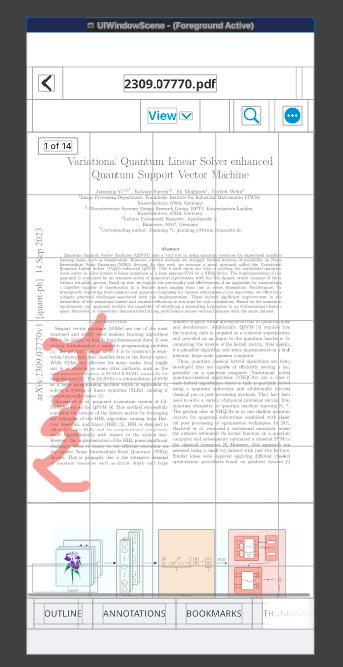
\includegraphics[width=0.5\textwidth]{Images/PdfTronViewController.png}
    \caption{PdfTronViewController ekranas}
    \label{fig:pdfViewController screen}
\end{figure}
\newpage
\subsection{Mobiliosios programėlės komponentų išskaidymas}

Programuojant mobiliasias progamėles, itin naudinga matyti, kokie komponentai buvo naudojami specifiniame mobiliosios programėlės lange. Tai leidžia greitai ir efektyviai identifikuoti, kurie komponentai yra naudojami ir kaip jie yra sukonfigūruoti.
\ref{img:pdfViewController} paveikslėlyje galime matyti, kaip atrodo \enquote{PdfTronView} dekompozicija, ekraną galima pasukti, norint pamatyti 3d dekompoziciją. Ieškant iškilusių problemų dideliame projekte, šis funkcionalumas yra labai naudingas, nes leidžia greitai rasti kokie komponentai naudojami, jų pavadinimus. 
\begin{figure}[htbp!]
    \centering
    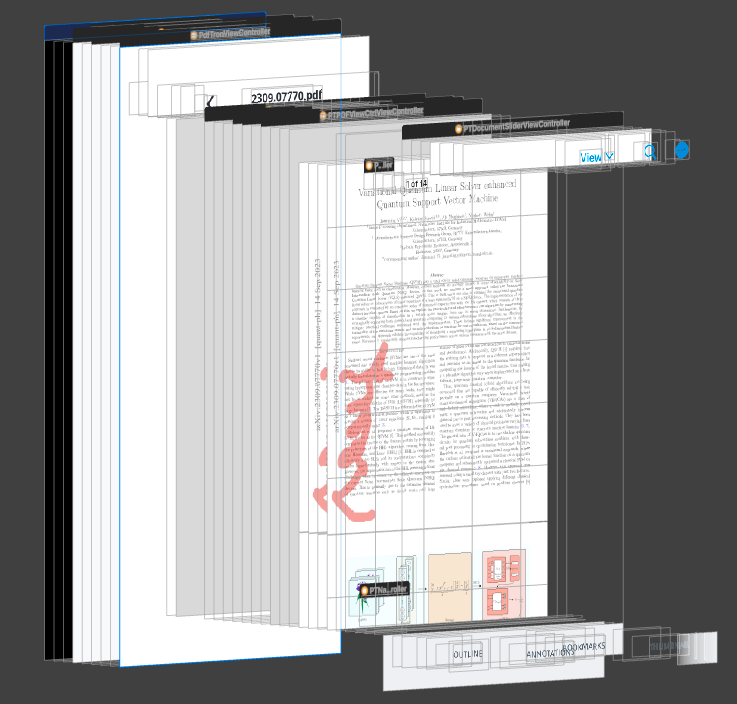
\includegraphics[width=0.8\textwidth]{Images/SideViewPdfViewController.png}
    \caption{PdfTronViewController dekompozicija}
    \label{img:pdfViewController}
\end{figure}
\newpage
\subsection{Anotacijų sąrašo PDF dokumente komponentas}
\enquote{PdfViewController} pavaizduoja dokumente esančias anotacijas, kurias galima redaguoti, ištrinti ar pridėti naujas.
 Taip pat yra galimybė pasirinkti anotacijos spalvą, dydį ir stilių. Esant dideliam anotacijų skaičiui, \enquote{AnnotationListViewController} pateikia anotacijų sąrašą, kurį galima filtruoti pagal anotacijos tipą, puslapį.
 Anotacijų sąraše galima pasirinkti anotaciją, kurią norima redaguoti, ištrinti ar peržiūrėti jos turinį ar sukurti naują formą. 
\begin{figure}[htbp!]
    \centering
    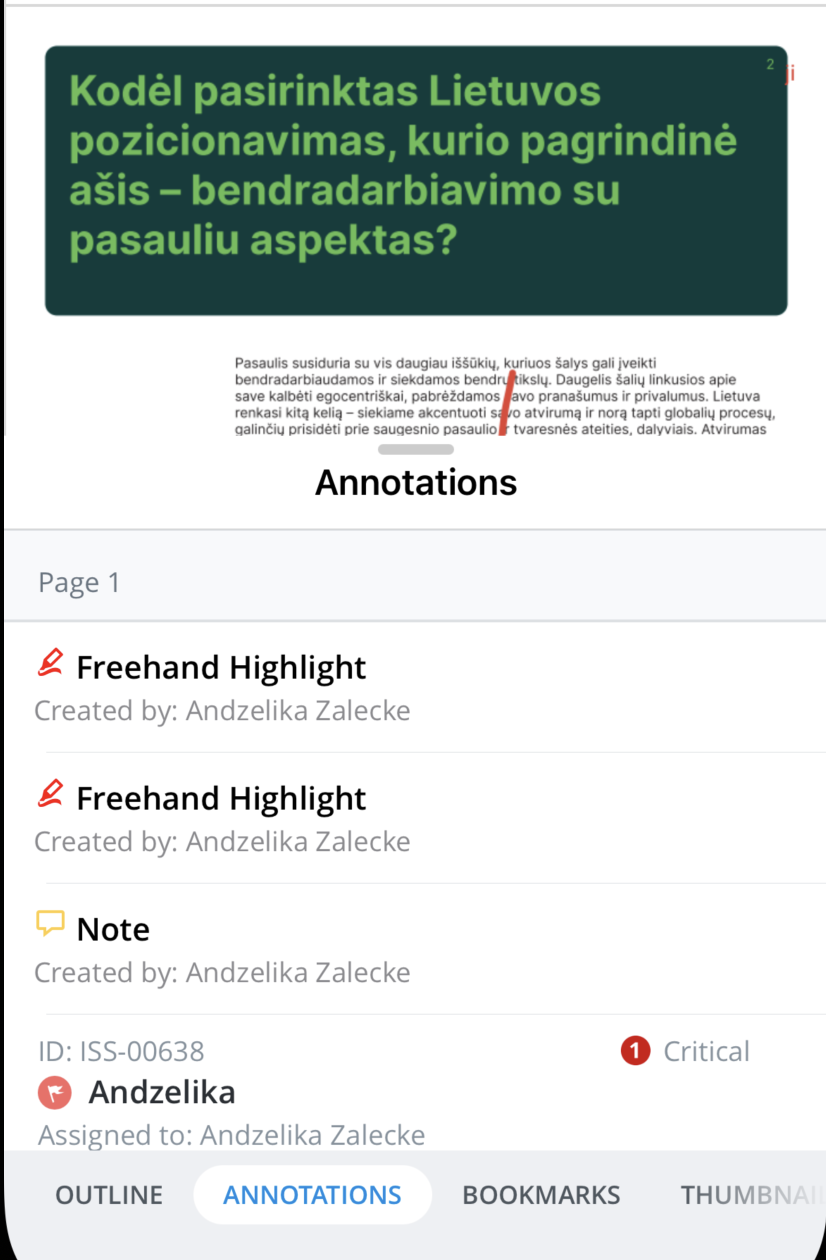
\includegraphics[width=0.6\textwidth]{Images/annotationList.png}
    \caption{Anotacijų sąrašo komponentas}
    \label{img:annotationList}
\end{figure}
\newpage
\subsection{Mobiliojoje programėlėje naudojamų mygtukų langas}
Projekte yra itin daug, įvairaus stiliaus mygtukų, atnaujinus iOS versiją ar programavimo karkasą, sunku pastebėti ar įvyko vizualūs pokyčiai. Tam buvo sukurtas Projekto mygtukų langas, kuriame galima matyti visus skirtingus, mygtukus programėlėje. 
Galima testuoti, kaip mygtukai reaguoja į įvairius veiksmus, kaip veikia jų animacijos, ar jie veikia pagal numatytą funkcionalumą. Visi mygtukai yra išdėstyti vienoje eilėje, todėl galima lengvai palyginti jų dydį, spalvą, formą ir kitas savybes. Mygtukų stiliaus nustatymas atnaujintas naudojant \enquote{UIButton.Configuration}, kuris leidžia paprastai, vienoje vietoje nustatyti specifinio mygtuko stilių. Senesni mygtukų stiliaus nustatymai buvo Storyboards, Swift kode.
Senesnis stiliaus nustatymo būdas turėjo problemų, nes ne visada buvo aišku, kur yra nustatymai, kurie nustato mygtuko stilių ir ar jie veikia. Naujasis būdas yra aiškesnis, nes visi nustatymai yra vienoje vietoje, lengvai prieinami ir aiškiai nurodyti.
\begin{figure}[htbp!]
    \centering
    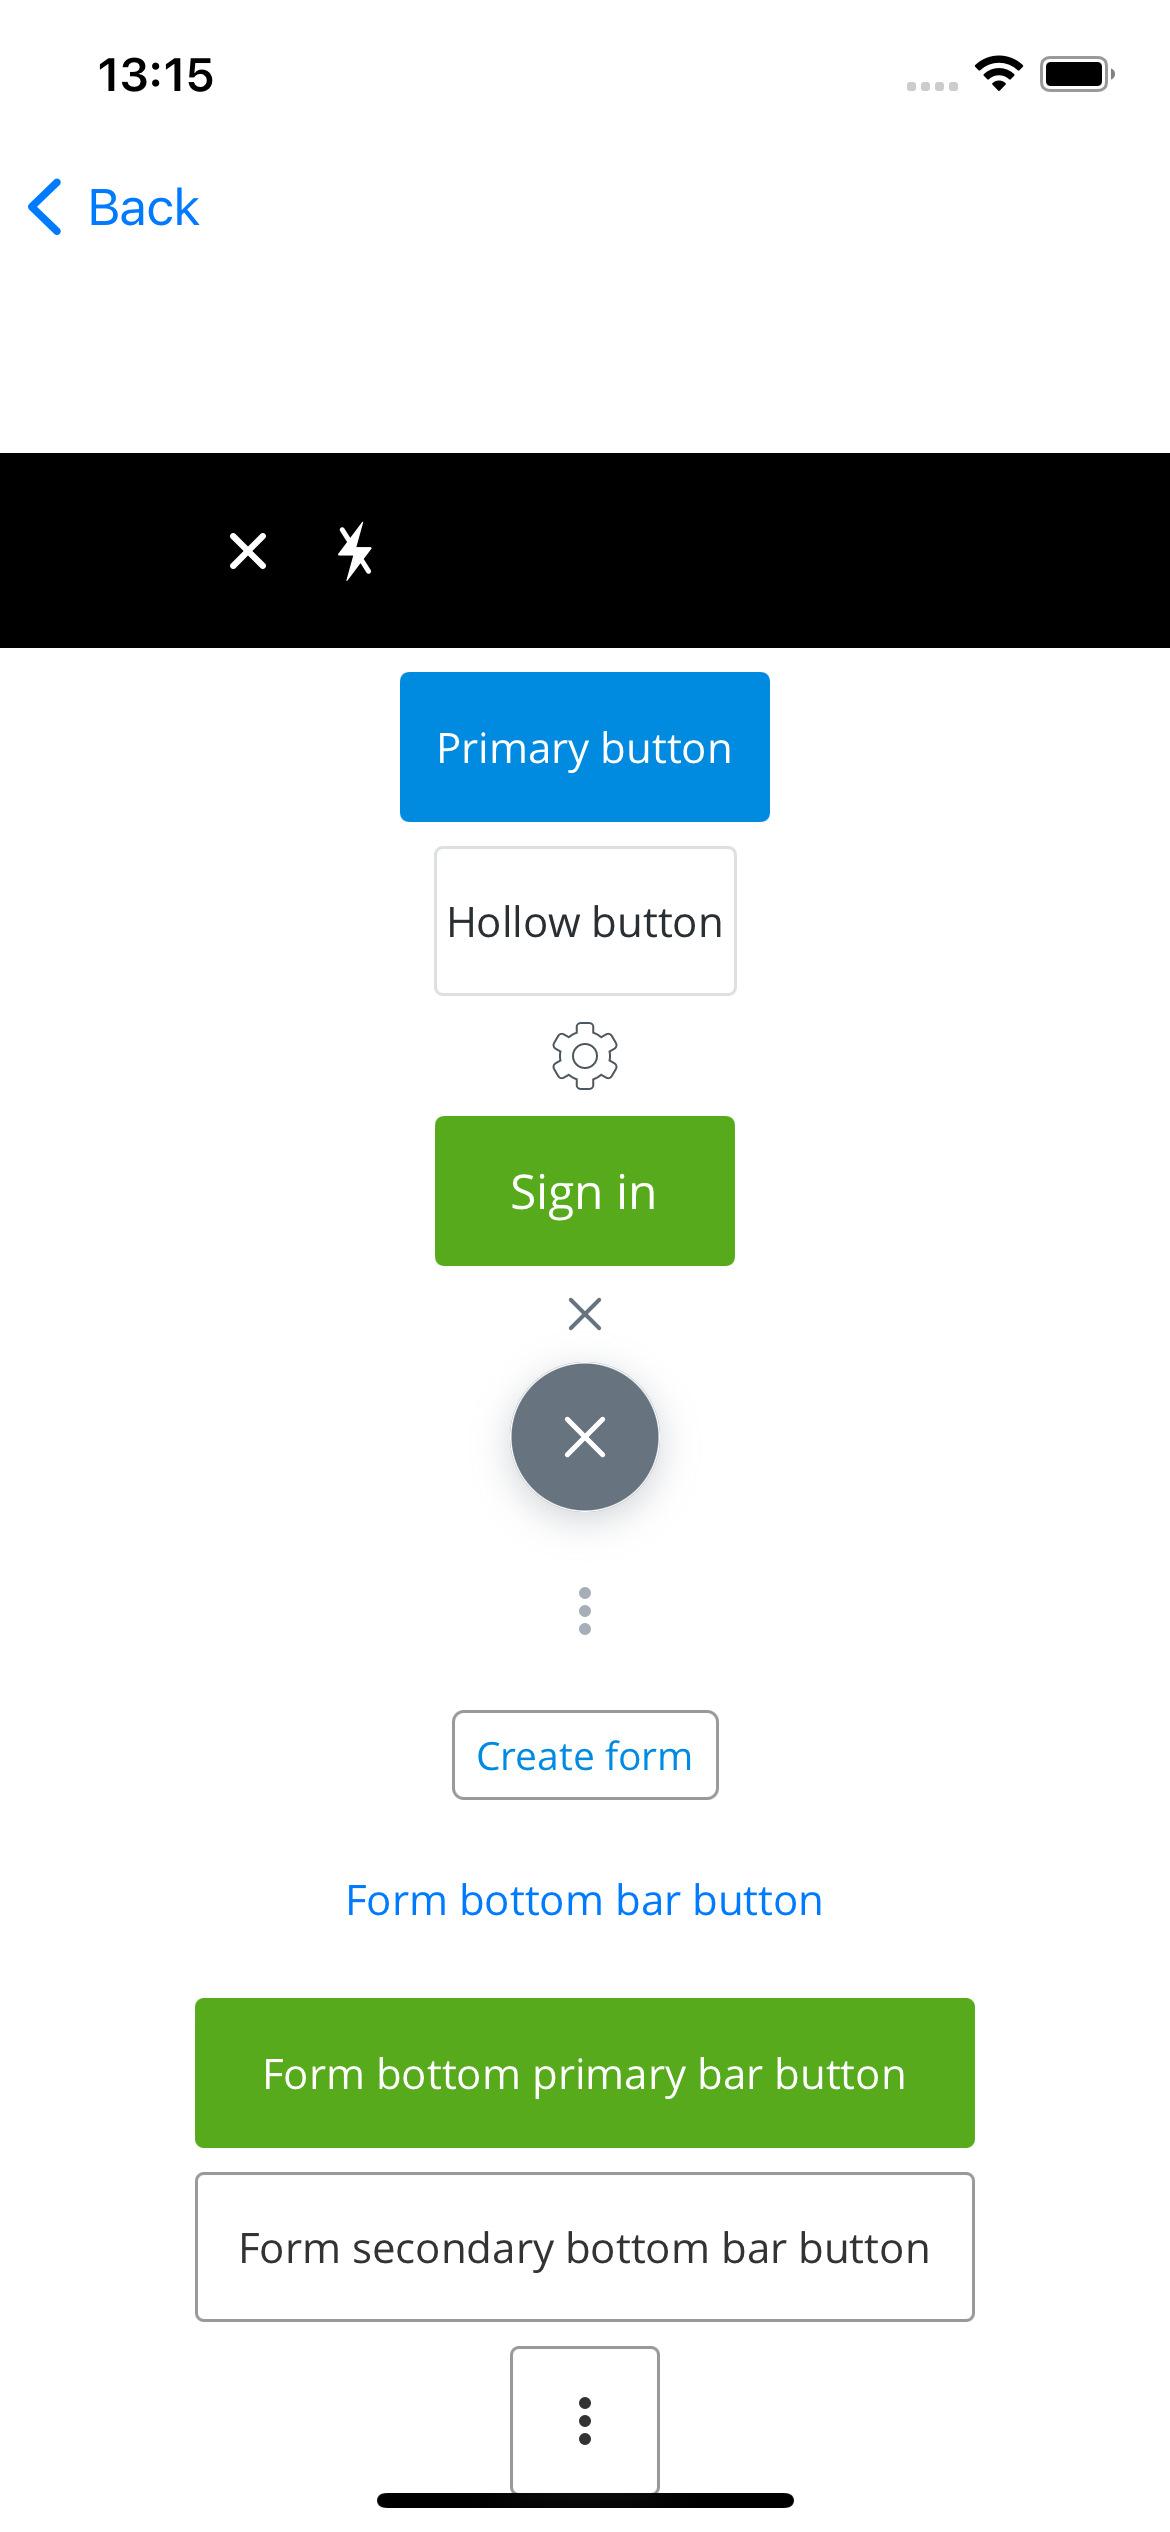
\includegraphics[width=0.4\textwidth]{Images/buttonsView.png}
    \caption{Projekto mygtukų langas}
    \label{fig:buttonsView.png}
\end{figure}
\newpage
\subsection{Vartotojo sąsajos komponentų programavimas naudojantis Jetpack compose karkasu}
Kadangi nuo 32 Android SDK versijos, Android pateikiamų iššokančių žinučių negalima keisti, nes tai turi tam tikrų saugumo spragų, buvo sukurtas naujas komponentas, pagal vartotojo sąsajos 
dizaino maketus. Jetpack Compose lengvai, net nepaleidus komponento įrenginyje, leidžia kurti vartotojo sąsajas, kurios atitinka naujausius dizaino standartus. Kiekvienas komponento pakeitimas iškart vizualiai matomas.
 Galima vizualiai pateikti vieno komponento visus testinius atvejus: Kai tekstas yra kelių eilučių, per ilgas ir pan. Taip pat galima pateikti, kaip komponentas elgiasi, kai jis yra įtrauktas į kitą komponentą.
  Yra galimybė sukurti įvairių dydžių ekranus, stebėti, kaip komponentas elgiasi, kiekvienu atveju. 

\begin{figure}[htbp!]
    \centering
    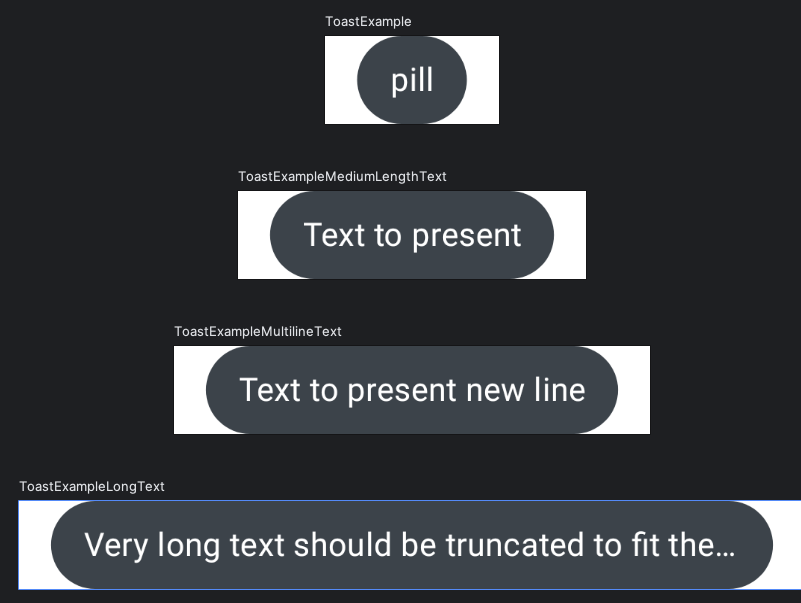
\includegraphics[width=0.7\textwidth]{Images/pillAndroid.png}
    \caption{Iššokančios žinutės komponentas}
    \label{fig:pill}
\end{figure}
\newpage
\subsection{Mobilioji programėlė su keleta pagrindinių langų}
Synchro Field mobilioji programėlė yra fragmentais grįsta su 2 pagrindiniais langais (\emph{angl. activities}). Toks dizaino sprendimas priimtas, nes virtualaus dvynio (\emph{angl. digital twin}) langas sukurtas kitos komandos. Šis komponentas yra
internetinio puslapio pobūdžio ir nėra tiesiogiai pritaikytas naudoti mobiliojoje programėlėje. Lengviausias būdas atvaizduoti, buvo sukurti atskirą pagrindinį langą, atlikti reikiamus pakeitimus ir atvaizduoti jį programėlėje.
 
 Norint pridėti iššokančios žinutės komponentą į 
programėlę, reikia sukurti ir pridėti komponentą į kiekvieną pagrindinį langą. Naudojamas tas pats viewModel objektas, kuris yra bendras visoms programėlės ekranams, norint, kad
iššokančių žinučių eilė būtų matoma visuose programėlės languose. 
\begin{figure}[htbp!]
    \centering
    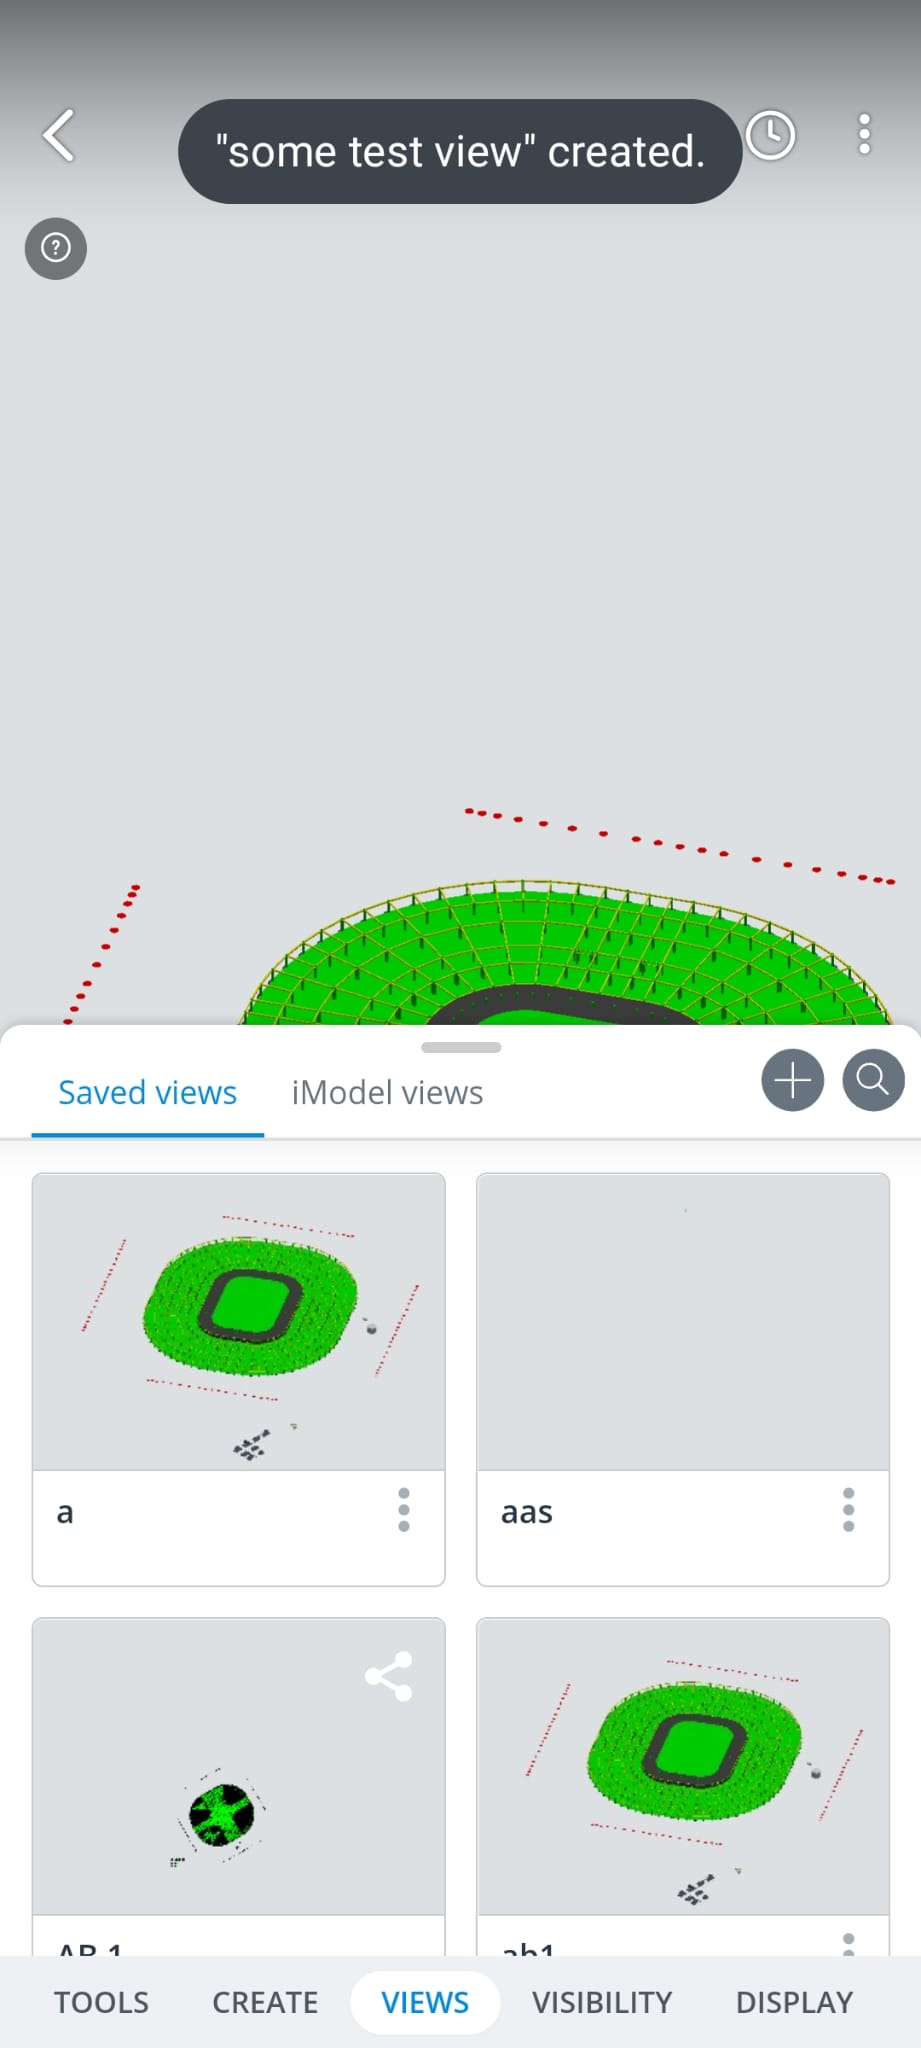
\includegraphics[width=0.45\textwidth]{Images/toastView.jpeg}
    \caption{Iššokančios žinutės komponento pavyzdys programėlėje}
    \label{fig:modelToastView}
\end{figure}